\chapter[]{Appendix example}

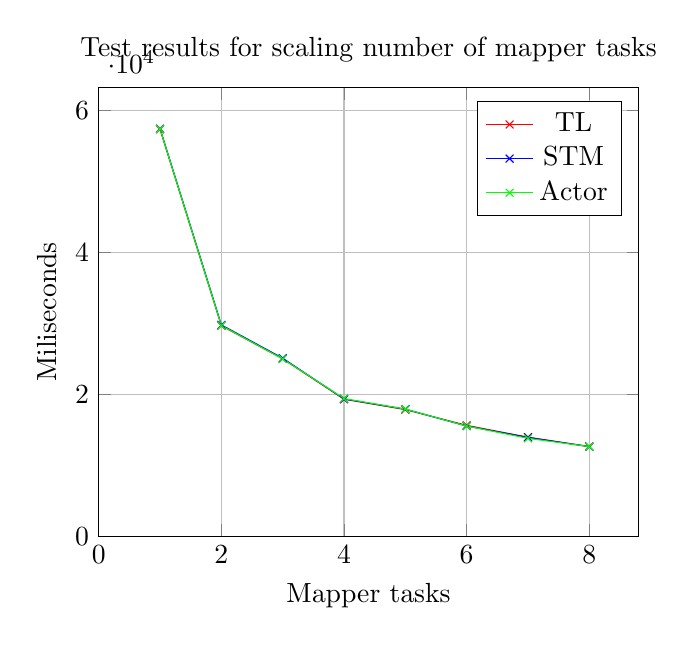
\begin{tikzpicture}
	\begin{axis}[
		legend entries={\acs{TL},\acs{STM}, Actor},
		legend pos=north east,
		grid = both,
		xlabel=Mapper tasks,
		ylabel=Miliseconds,
		xmin=0,
		ymin=0, 
		title=Test results for scaling number of mapper tasks,
		label=fig:tr_scale_mappers]		
	\addplot[color=red,mark=x] coordinates {
		(1,57294)
		(2,29625)
		(3,24969)
		(4,19290)
		(5,17823)
		(6,15611)
		(7,13930)
		(8,12637)
	};
	\addplot[color=blue,mark=x] coordinates {
		(1,57388)
		(2,29749)
		(3,25068)
		(4,19319)
		(5,17890)
		(6,15506)
		(7,13919)
		(8,12599)
	};
	\addplot[color=green,mark=x] coordinates {
		(1,57343)
		(2,29660)
		(3,24970)
		(4,19378)
		(5,17897)
		(6,15512)
		(7,13773)
		(8,12617)
	};
	\end{axis}
\end{tikzpicture}

\begin{center}
\begin{table}[h]
\centering
\begin{tabular}{c|ccc}
\# Mapper tasks 	& \ac{TL}   & \ac{STM}   & Actor \\ \hline
1                   &     57294      &      57388      &    57343   \\
2                   &     29625      &      29749      &    29660   \\
3                   &     24969      &      25068      &    24970   \\
4                   &     19290      &      19319      &    19378   \\
5                   &     17823      &      17890      &    17897   \\
6                   &     15611      &      15506      &    15512   \\
7                   &     13930      &      13919      &    13773  \\
8                   &     12637      &      12599      &    12617  
\end{tabular}
\end{table}
\label{table:test_results_concurrent_tasks}
\end{center}


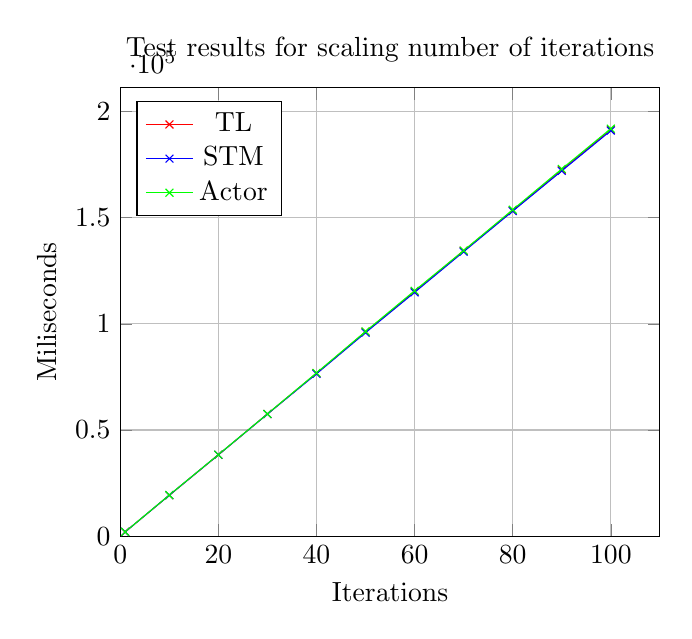
\begin{tikzpicture}
	\begin{axis}[
		legend entries={\acs{TL},\acs{STM}, Actor},
		legend pos=north west,
		grid = both,
		xlabel=Iterations,
		ylabel=Miliseconds,
		xmin=0,
		ymin=0, 
		title=Test results for scaling number of iterations,
		label=fig:tr_scale_iterations]		
	\addplot[color=red,mark=x] coordinates {
		(1,2019)
		(10,19290)
		(20,38312)
		(30,57537)
		(40,76701)
		(50,96235)
		(60,115203)
		(70,134404)
		(80,153350)
		(90,172521)
		(100,191413)
	};
	\addplot[color=blue,mark=x] coordinates {
		(1,2017)
		(10,19319)
		(20,38328)
		(30,57508)
		(40,76480)
		(50,95854)
		(60,114832)
		(70,133984)
		(80,153082)
		(90,172041)
		(100,190996)
	};
	\addplot[color=green,mark=x] coordinates {
		(1,2027)
		(10,19378)
		(20,38390)
		(30,57578)
		(40,76877)
		(50,96398)
		(60,115575)
		(70,134495)
		(80,153730)
		(90,172925)
		(100,191914)
	};
	\end{axis}
\end{tikzpicture}


\begin{center}
\begin{table}[h]
\centering
\begin{tabular}{c|ccc}
\# Iterations 	& \ac{TL}   & \ac{STM}   & Actor \\ \hline
1  	& 	   	 2019		&      2017		&		2027       \\
10	&     19290		&      19319		&		19378       \\
20	&     38312		&      38328		&		38390       \\
30	&		57537		&      57508		&		57578       \\
40	&		76701		&      76480		&		76877       \\
50	&		96235		&      95854 	&		96398       \\
60  	&     115203	&      114832	&		115575       \\
70	&     134404	&      133984	&		134495       \\
80	&		153350	&      153082	&		153730       \\
90	&		172521	&      172041	&		172925       \\
100	&		191413	&      190996	&		191914      
\end{tabular}
\end{table}
\label{table:test_results_iterations}
\end{center}

\end{lstlisting}